% % % % % % % % % % % % % % % % % % % % % % % % % % % % % % % % % % % % % % % % % % % %
%                                                                                     %
% Short Sectioned Assignment LaTeX Template Version 1.0 (5/5/12)                      %
% This template has been downloaded from: http://www.LaTeXTemplates.com               %
%                                                                                     %
% Original author:  Frits Wenneker (http://www.howtotex.com)                          %
%                                                                                     %
% Modified by: Fco Javier Sueza Rodríguez (fcosueza@disroot.org)                      %
%                                                                                     %
% Changes:                                                                            %
%	    - Custom Chapters, Sections and Subsections (titlesec package)                %
%           - Document type scrbook (oneside)                                         %
%           - Use babel-lang-spanish package and marvosym                             %
%           - Use hyperref, enumitem, tcolorbox and glossaries packages               %
%           - Use Time New Roman (mathptmx), Helvetic and Courier fonts               %
%                                                                                     %
% License: CC BY-NC-SA 3.0 (http://creativecommons.org/licenses/by-nc-sa/3.0/)        %
%                                                                                     %
% % % % % % % % % % % % % % % % % % % % % % % % % % % % % % % % % % % % % % % % % % % %

%-----------------------------------------------%
%	              Packages                  %
%-----------------------------------------------%

\documentclass[paper=a4, fontsize=11pt, oneside]{scrbook}

% ---- Text Input/Output ----- %

\usepackage[T1]{fontenc}
\usepackage[utf8]{inputenc}
\usepackage{mathptmx}
\usepackage[scaled=.92]{helvet}
\usepackage{courier}
\usepackage[indent=12pt]{parskip}

\usepackage{geometry}
\geometry{verbose,tmargin=3cm,bmargin=3cm,lmargin=2.6cm,rmargin=2.6cm}

% ---- Language ----- %

\usepackage[spanish]{babel}
\usepackage{marvosym}

% ---- Another packages ---- %

\usepackage{amsmath,amsfonts,amsthm}
\usepackage{graphics,graphicx}
\usepackage{titlesec}
\usepackage{fancyhdr}
\usepackage{tcolorbox}
\usepackage{hyperref}
\usepackage{enumitem}
\usepackage[automake]{glossaries}

%--------------------------------------------------------------------%
%                      Customizing Document                          %
%--------------------------------------------------------------------%


% ----------- Custom Chapters, Sections and Subsections -------------- %

\titleformat{\chapter}[display]
			{\bfseries\Huge}
			{Tema \ \thechapter} {0.5ex}
			{\vspace{1ex}\centering}

\titleformat{\section}[hang]
			{\bfseries\Large}
			{\thesection}{0.5em}{}

\titleformat{\subsection}[hang]
			{\bfseries\large}
			{\thesubsection}{0.5em}{}

\titleformat{\subsubsection}[hang]
			{\bfseries\large}
			{\thesubsubsection}{0.5em}{}

\hypersetup{
    colorlinks=true,
    linkcolor=black,
    urlcolor=magenta
}

% ------------------- Custom heaaders and footers ------------------- %

\pagestyle{fancyplain}

\fancyhead[]{}
\fancyfoot[L]{}
\fancyfoot[C]{}
\fancyfoot[R]{\thepage}

\renewcommand{\headrulewidth}{0pt} % Remove header underlines
\renewcommand{\footrulewidth}{0pt} % Remove footer underlines

\setlength{\headheight}{13.6pt} % Customize the height of the header

% --------- Numbering equations, figures and tables ----------------- %

\numberwithin{equation}{section} % Number equations within sections
\numberwithin{figure}{section} % Number figures within sections
\numberwithin{table}{section} % Number tables within sections

% ------------------------ New Commands ----------------------------- %

\newcommand{\horrule}[1]{\rule{\linewidth}{#1}} % Create horizontal rule command


%----------------------------------------------------------------------------------------
%	TÍTULO Y DATOS DEL ALUMNO
%----------------------------------------------------------------------------------------

\title{
\vspace{10ex}
\normalfont \normalsize
\Huge \textbf{Tarea 4: Instalación y Configuración de Windows (I)}
}
\author{Francisco Javier Sueza Rodríguez}
\date{\normalsize\today}

%----------------------------------------------------------------------------------------
%                                     DOCUMENTO
%----------------------------------------------------------------------------------------
\begin{document}

\maketitle

\thispagestyle{empty}

\vspace{68ex}

\begin{center}
    \begin{tabular}{l l}
        \textbf{Centro}: & IES Aguadulce \\
        \textbf{Ciclo Formativo}: & Desarrollo Aplicaciones Web (Distancia)\\
        \textbf{Asignatura}: & Sistemas Informáticos\\
        \textbf{Tema}: & Tema 4 -  Instalación y Configuración de Windows (I)\\
    \end{tabular}
\end{center}

\newpage

\tableofcontents

\newpage

\listoffigures

\newpage

\section{Caso Práctico}
Ada le encarga a María y a Juan que configure los equipos de la empresa AguadulSoft, según las preferencias de los usuarios y usuarias, con Windows 10 y Windows 8.1. Su objetivo es configurar en el equipo los dos sistemas operativos y realizar las configuraciones básicas del sistema.

\section{Actividades}

\subsection{Actividad 1: Preparación del Software de Virtualización}

\subsubsection{Enunciado}
Descarga e instala la última versión de VMware Workstation Player (recomendado) o VirtualBox que sea la adecuada para el sistema operativo que utilices en tu ordenador. Si lo tienes ya instalado en tu ordenador y no es la última versión, actualízalo. Recomendamos el uso de VMware por posibles problemas de compatibilidad en tareas posteriores del módulo.

\textbf{Capturas}:

\begin{itemize}
    \item Página de descarga del software de virtualización (en caso de actualización, mensaje que indica que hay una actualización disponible).
    \item Inicio del proceso de instalación.
    \item Fin del proceso de instalación (cuando nos informa que ha sido correctamente instalado), donde se debe ver la versión que se ha instalado.
\end{itemize}

\textbf{NOTA}: Si ya tienes la última versión instalada puedes volver a instalarlo, o bien mostrar la página de descarga, luego el inicio del instalador, y luego cancelar la instalación y mostrar el programa ya ejecutándose en la ventana ``Acerca de...'', donde se muestra la versión del programa.

\subsubsection{Solución}

\begin{enumerate}
    \item En primer lugar hemos accedido a la \href{https://customerconnect.vmware.com/en/downloads/details?downloadGroup=WKST-PLAYER-1701&productId=1377&rPId=100675}{página de descarga} de WMWare y hemos descargado la versión 17.0.1 para Linux de 64-bits. Vamos a usar VMWare, aunque ya teníamos instalado VirtualBox para otra asignatura, para ahorrarnos problemas de compatibilidad tal y como se recomienda en la descripción de la tarea.

    \begin{figure}[H]
        \centering
        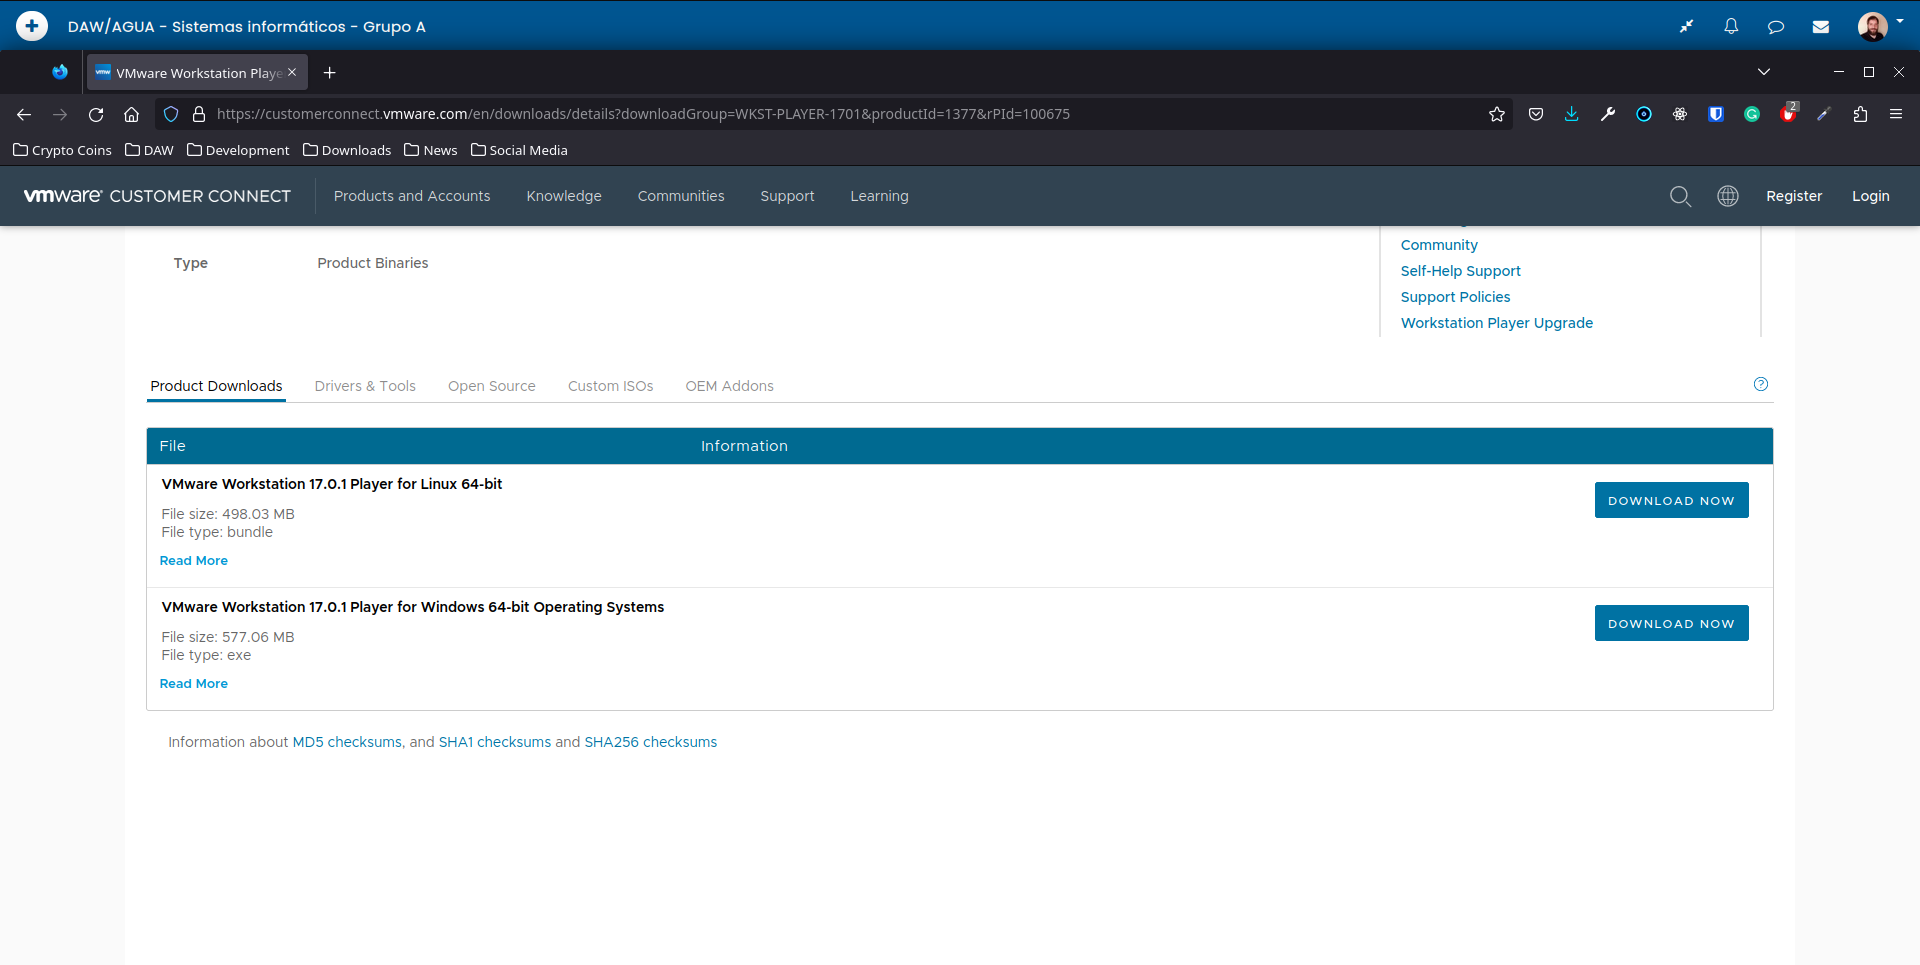
\includegraphics[scale=0.23]{vmware-download.png}
        \caption{Página de descarga de VMWare Workstation}
    \end{figure}

    \item A continuación hemos ejecutado el script que se nos ha proporcionado y que instalará el bundle de VMWare. En la siguiente captura se puede ver el script ejecutándose en una terminal y realizando la instalación de los paquetes.

    \begin{figure}[ht]
        \centering
        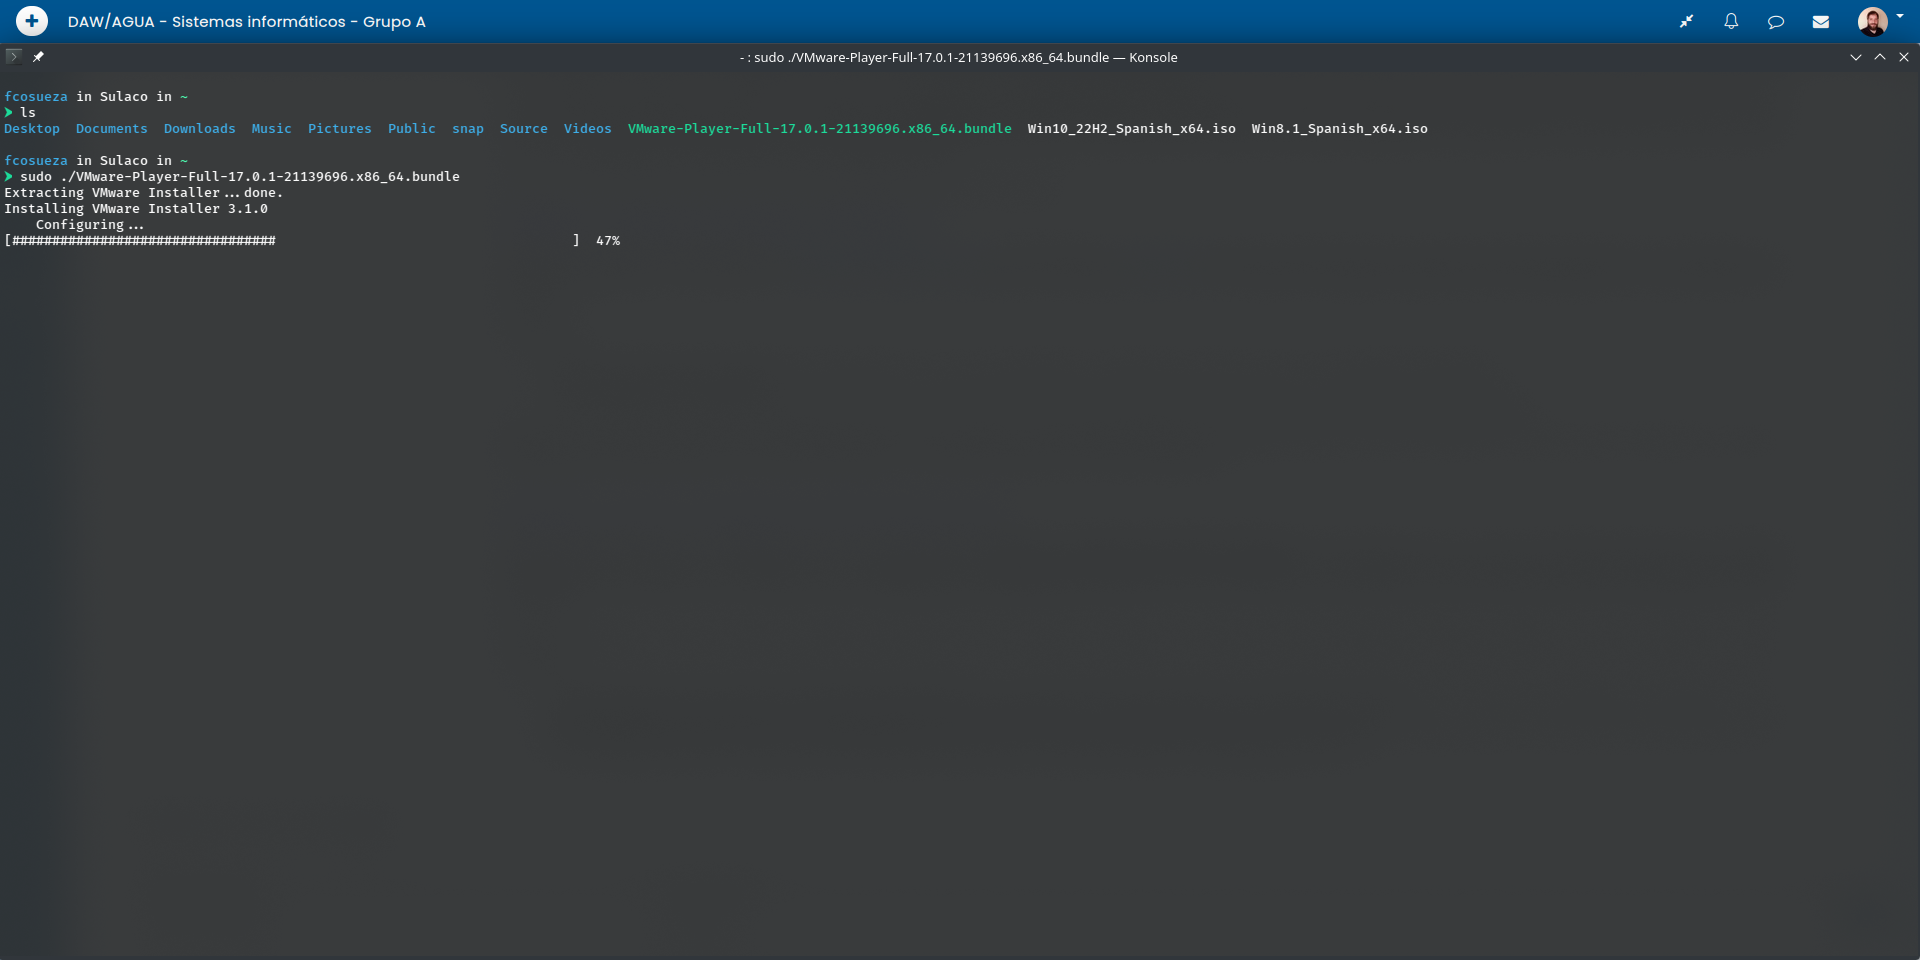
\includegraphics[scale=0.23]{vmware-install.png}
        \caption{Instalación de VMWare Workstation}
    \end{figure}

    \item Después de realizar la instalación desde la terminal y tras abrir por primera vez la aplicación, se nos da la opción de personalizar la instalación, aunque nosotros no hemos realizado ninguna modificación en esta. En la siguiente captura se muestra esta ventana.

    \begin{figure}[ht]
        \centering
        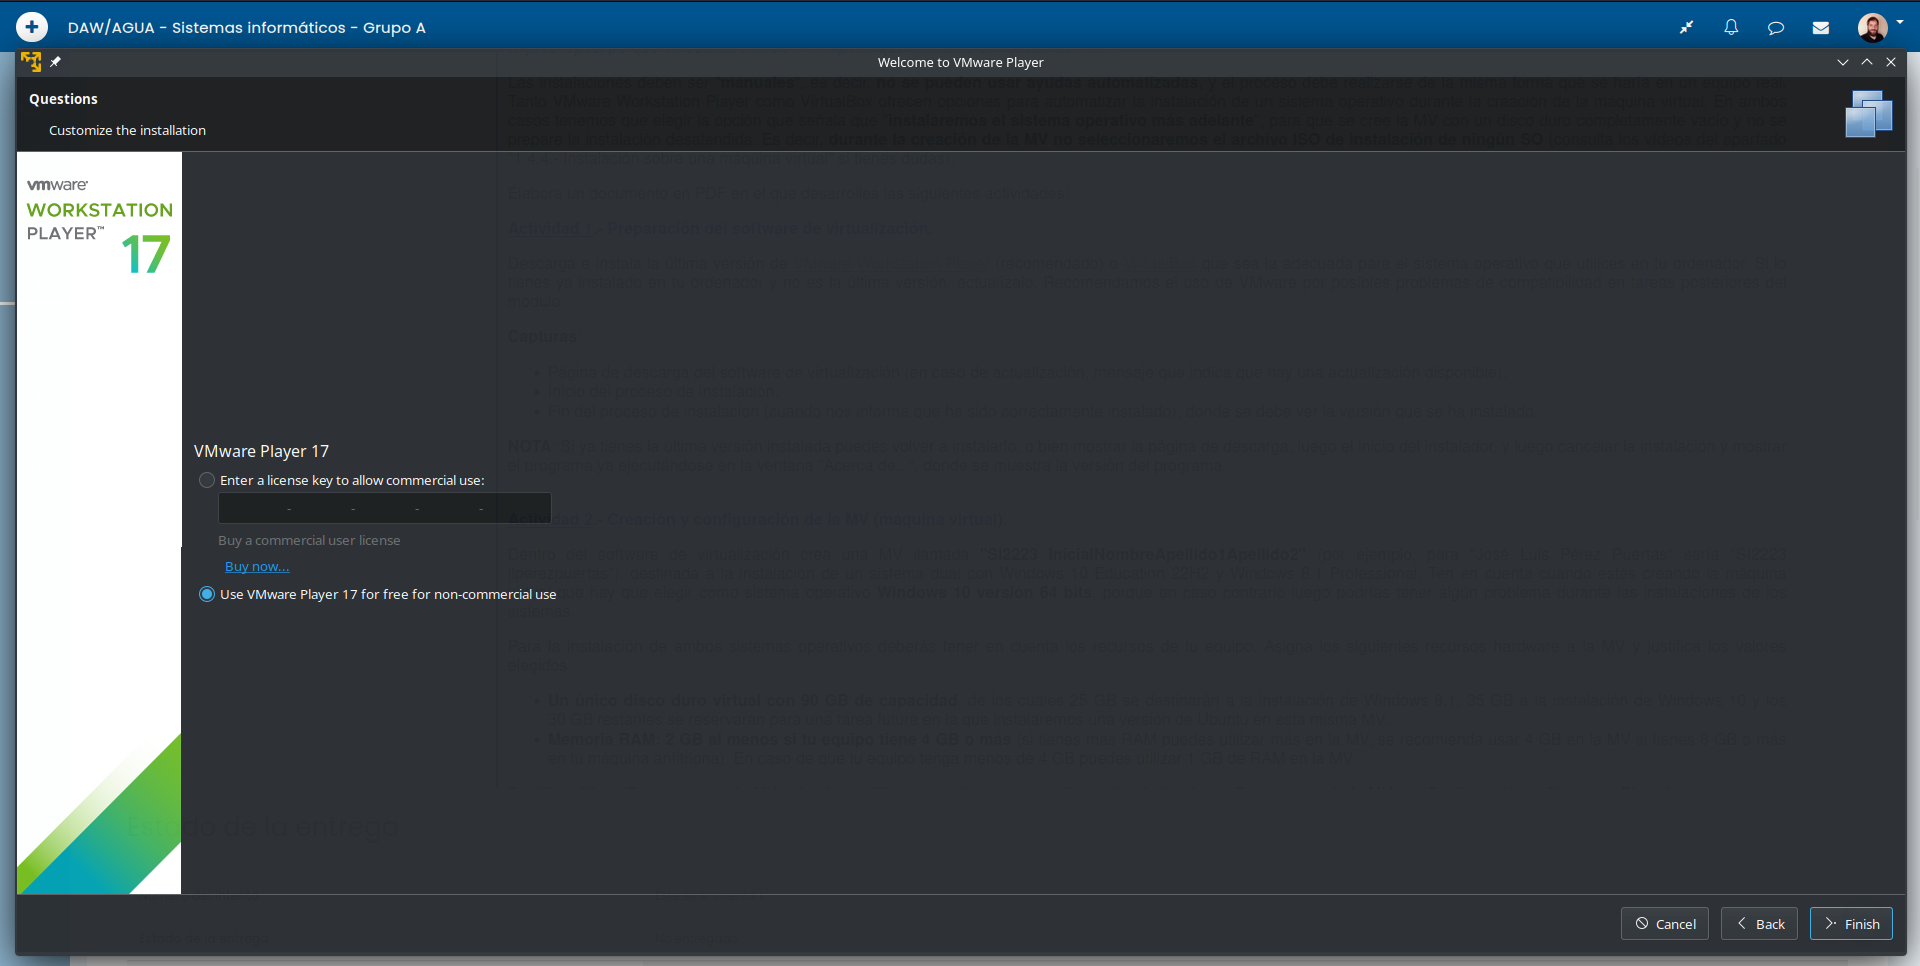
\includegraphics[scale=0.23]{vmware-install-2.png}
        \caption{Personalización de la Instalación de VMWare}
    \end{figure}

    \item Una vez llevado a cabo estos pasos, ya tenemos realizada la instalación de VMWare en Ubuntu. En la siguiente captura, podemos ver la máquina virtual instalada y sus especificaciones, así como la del host. Aunque en este portátil tengo 8 GB de RAM, la tarjeta gráfica no tiene memoria dedicada, por lo que 2 Gb de estos 8 están reservados para ese propósito, como muestra esta ventana, aunque ya hablaremos de esto en la siguiente sección.

    \begin{figure}[ht]
        \centering
        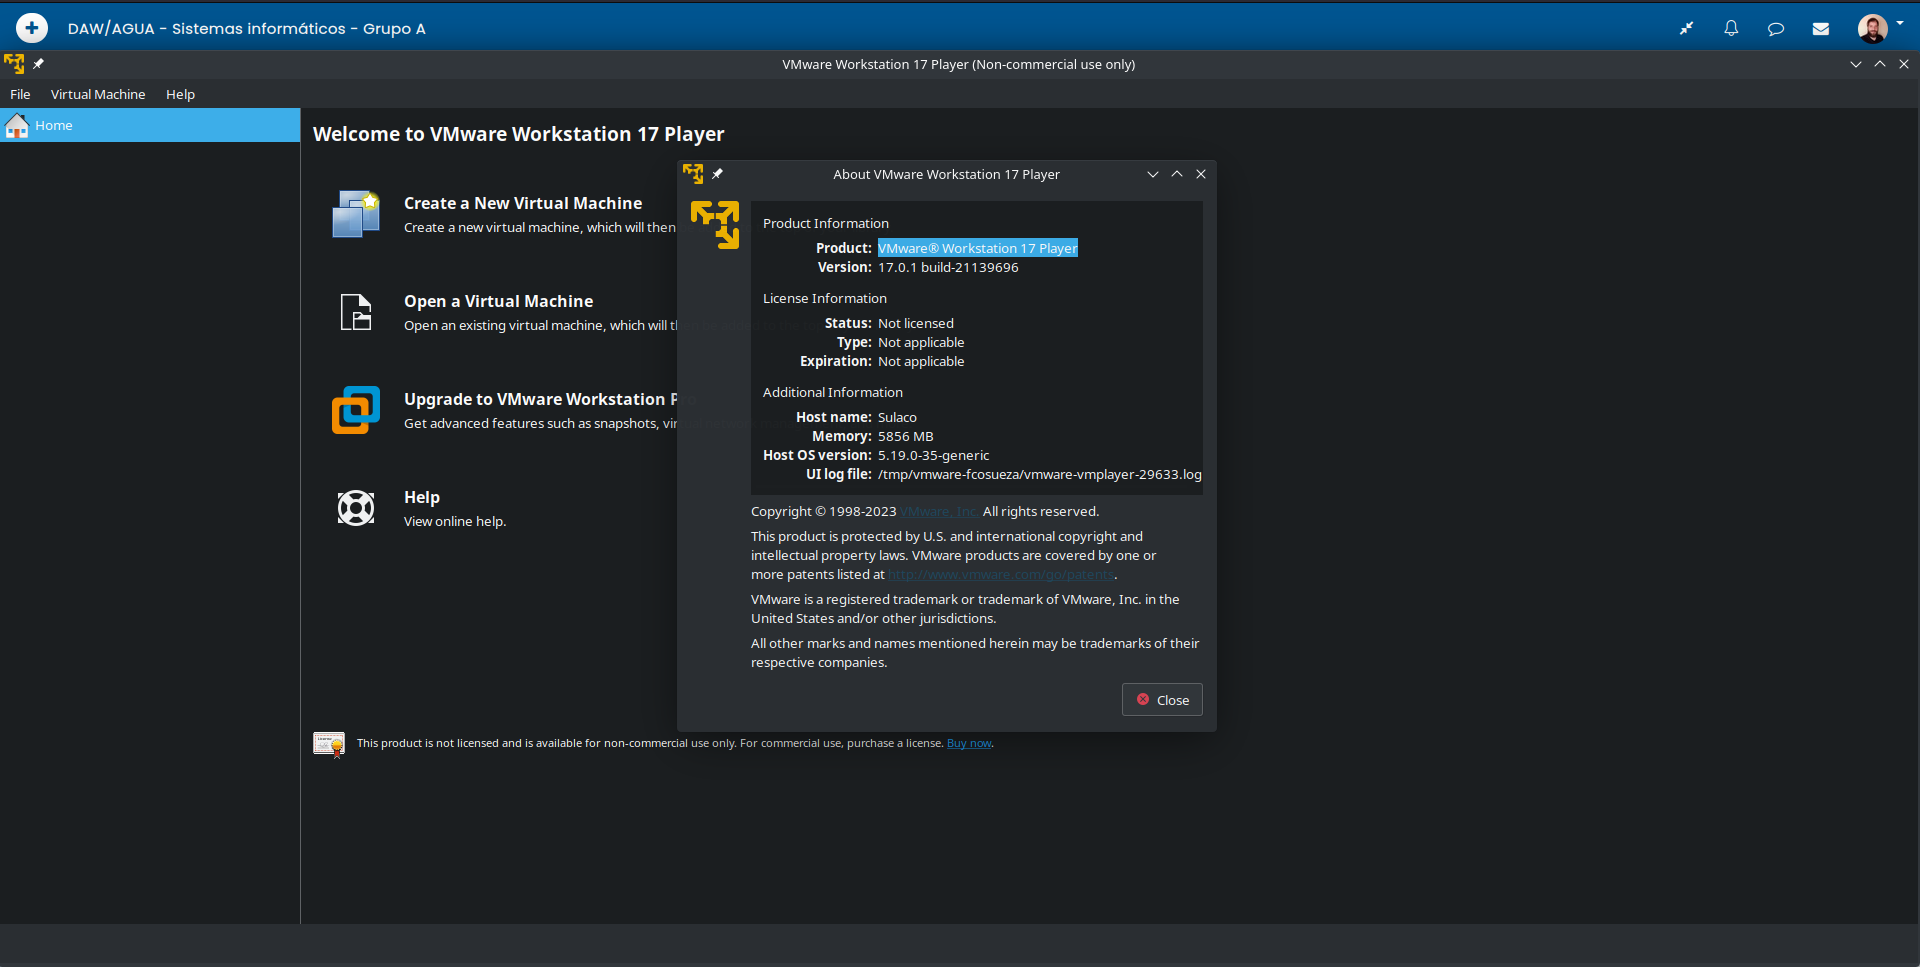
\includegraphics[scale=0.23]{vmware-install-3.png}
        \caption{Ventana de información sobre la versión instalada de VMWare}
    \end{figure}
\end{enumerate}

\subsection{Actividad 2}

\subsection{Enunciado}
Dentro del software de virtualización crea una MV llamada ``SI2223 InicialNombreApellido1Apellido2'' (por ejemplo, para ``José Luis Pérez Puertas'' sería ``SI2223 jlperezpuertas''), destinada a la instalación de un sistema dual con Windows 10 Education 22H2 y Windows 8.1 Professional. Ten en cuenta cuando estés creando la máquina virtual que hay que elegir como sistema operativo Windows 10 versión 64 bits, porque en caso contrario luego podrías tener algún problema durante las instalaciones de los sistemas.

Para la instalación de ambos sistemas operativos deberás tener en cuenta los recursos de tu equipo. Asigna los siguientes recursos hardware a la MV y justifica los valores elegidos:

\begin{itemize}
    \item \textbf{Un único disco duro virtual con 90 GB de capacidad}, de los cuales 25 GB se destinarán a la instalación de Windows 8.1, 35 GB a la instalación de Windows 10 y los 30 GB restantes se reservarán para una tarea futura en la que instalaremos una versión de Ubuntu en esta misma MV.

    \item \textbf{Memoria RAM: 2 GB al menos si tu equipo tiene 4 GB o más}, (si tienes más RAM puedes utilizar más en la MV, se recomienda usar 4 GB en la MV si tienes 8 GB o más en tu máquina anfitriona). En caso de que tu equipo tenga menos de 4 GB puedes utilizar 1 GB de RAM en la MV.
\end{itemize}


Si utilizas VirtualBox, tras crear la MV deberás modificar un parámetro de configuración de la misma. Entra dentro de la MV en ``Configuración > Sistema > Placa base'' y marca la opción ``Habilitar EFI''. Esto hará que la MV utilice un firmware de tipo UEFI, tal como es común en los equipos reales actuales.

\textbf{Capturas}

\begin{itemize}
    \item Introducción del nombre de la máquina y elección de tipo ``Windows 10 64 bits''.
    \item Cantidad de RAM asignada.
    \item Tamaño de disco duro asignado.
    \item Resumen con los datos de la máquina virtual creada en la ventana principal del programa de virtualización (en VirtualBox se debe ver en ``Sistema'' la opción ``EFI: Habilitado'').
\end{itemize}

\subsubsection{Solución}







% Bibliography
\newpage
\bibliography{citas}
\bibliographystyle{unsrt}

\end{document}